% Fig. 8 面向运营的决策流程：样本数  $\times$  纯度  $\times$  部署先验 → 选择（TikZ 示意图）；编译：pdflatex fig8_decision.tex
% 每个结论框都标注了支撑它的图：Fig. 5、6、7，附录 D（Westermo）
\documentclass[10pt]{standalone}
% 全部论文图共用的样式（颜色固定跟随来源；字号按 elsarticle 正文 10pt 设定）
% 颜色来自经过色觉校验的分类调色板，顺序固定：
%   类别权重 = 1 蓝，ROS = 2 橙，SMOTE = 3 青，Qwen = 4 黄，Llama = 5 品红；不增强 = 中性灰
\usepackage{pgfplots}
\usepgfplotslibrary{groupplots}
\pgfplotsset{compat=1.18}
\usetikzlibrary{plotmarks,calc,patterns,arrows.meta,positioning,shapes.geometric,fit,backgrounds}
\definecolor{cCW}{HTML}{2A78D6}
\definecolor{cROS}{HTML}{EB6834}
\definecolor{cSMOTE}{HTML}{1BAF7A}
\definecolor{cQWEN}{HTML}{EDA100}
\definecolor{cLLAMA}{HTML}{E87BA4}
\definecolor{cNONE}{HTML}{52514E}
\definecolor{cGRID}{HTML}{E4E3DF}
\definecolor{cAXIS}{HTML}{8A8984}
\definecolor{cTEXT}{HTML}{2B2A28}
\pgfplotsset{
  paper/.style={
    font=\footnotesize, color=cTEXT,
    axis line style={cAXIS, line width=0.4pt},
    tick style={cAXIS, line width=0.4pt},
    major tick length=2pt,
    grid style={cGRID, line width=0.4pt},
    ymajorgrids,
    tick label style={font=\scriptsize},
    label style={font=\footnotesize},
    title style={font=\footnotesize\bfseries, yshift=-2pt},
    legend style={font=\scriptsize, draw=none, fill=none, /tikz/every even column/.append style={column sep=8pt}},
    legend cell align=left,
  },
  errbar/.style={error bars/.cd, y dir=both, y explicit,
    error bar style={line width=0.5pt, cTEXT!75}, error mark options={rotate=90, mark size=1.4pt, line width=0.5pt, cTEXT!75}},
}

\definecolor{cFULL}{HTML}{008300}
\begin{document}
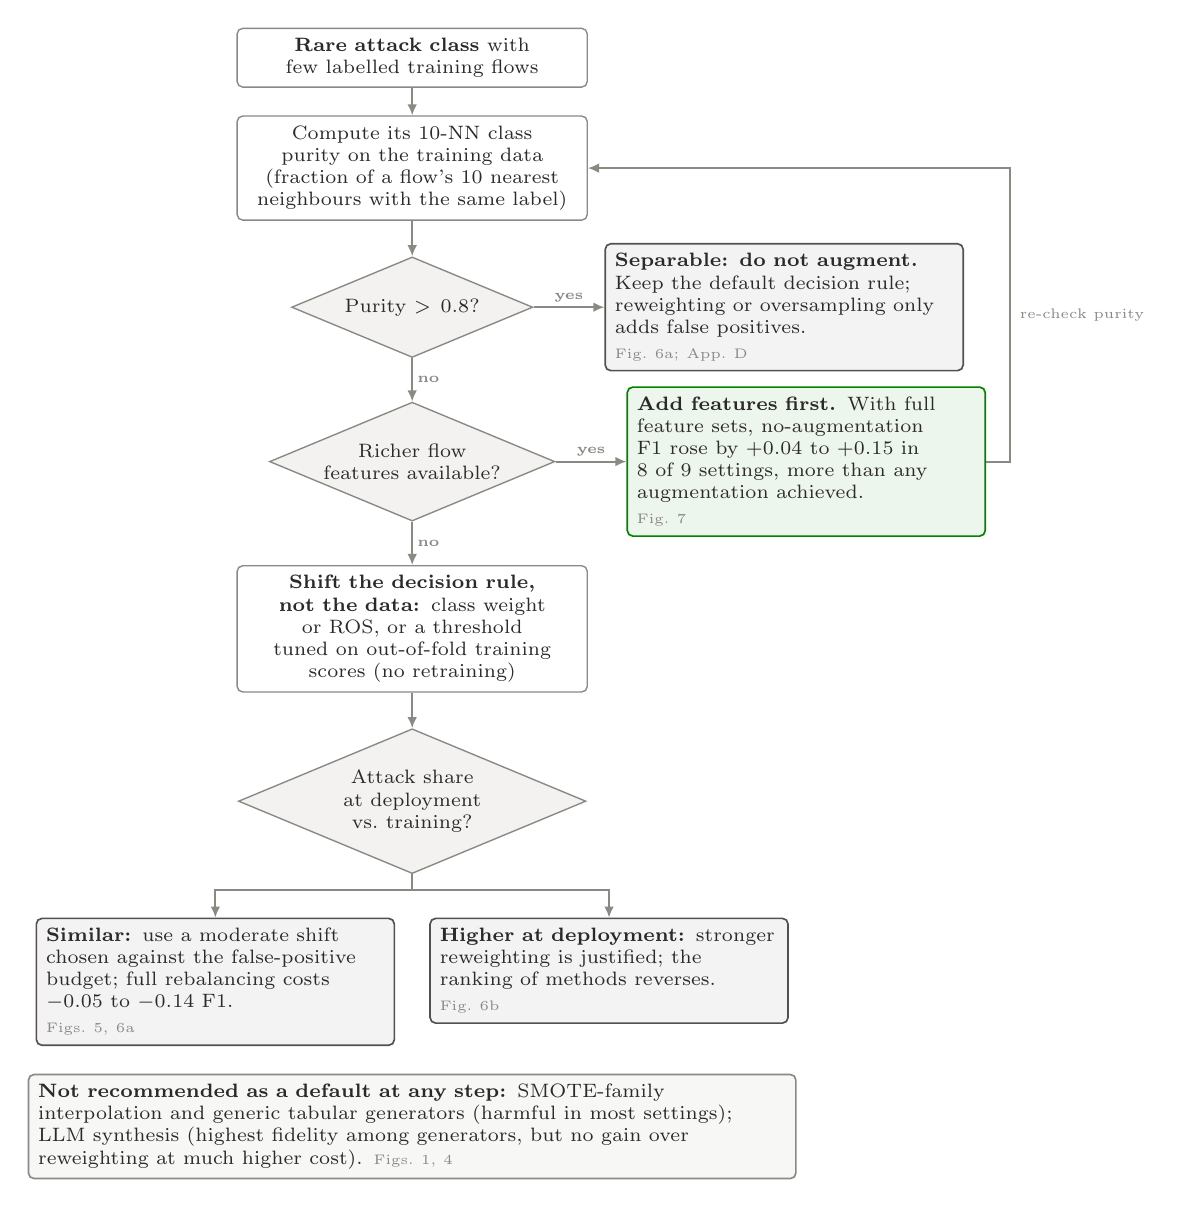
\begin{tikzpicture}[
  font=\scriptsize, color=cTEXT,
  every node/.append style={execute at begin node={\hyphenpenalty=10000\exhyphenpenalty=10000}},
  proc/.style={draw=cAXIS, line width=0.5pt, rounded corners=2pt, fill=white, align=center, inner sep=3.5pt, text width=#1},
  proc/.default=4.2cm,
  dec/.style={draw=cAXIS, line width=0.5pt, diamond, aspect=2.4, fill=cGRID!45, align=center, inner sep=1pt, text width=2.3cm},
  out/.style={draw=#1, line width=0.6pt, rounded corners=2pt, fill=#1!7, align=left, inner sep=3.5pt, text width=4.3cm},
  arr/.style={-{Latex[length=4pt, width=3.5pt]}, cAXIS, line width=0.7pt},
  yn/.style={font=\tiny\bfseries, cAXIS, inner sep=1.5pt},
  ref/.style={font=\tiny, cAXIS},
]
\node[proc] (start) {\textbf{Rare attack class} with few labelled training flows};
\node[proc, below=0.35cm of start] (purity) {Compute its 10-NN class purity on the training data (fraction of a flow's 10 nearest neighbours with the same label)};
\node[dec, below=0.45cm of purity] (q1) {Purity $> 0.8$?};
\node[out=cNONE, right=0.9cm of q1] (sep) {\textbf{Separable: do not augment.} Keep the default decision rule; reweighting or oversampling only adds false positives.\\[1pt]{\color{cAXIS}\tiny Fig.~6a; App.~D}};
\node[dec, below=0.55cm of q1] (q2) {Richer flow features available?};
\node[out=cFULL, right=0.9cm of q2] (feat) {\textbf{Add features first.} With full feature sets, no-augmentation F1 rose by $+0.04$ to $+0.15$ in 8 of 9 settings, more than any augmentation achieved.\\[1pt]{\color{cAXIS}\tiny Fig.~7}};
\node[proc, below=0.55cm of q2] (rew) {\textbf{Shift the decision rule, not the data:} class weight or ROS, or a threshold tuned on out-of-fold training scores (no retraining)};
\node[dec, below=0.45cm of rew] (q3) {Attack share at deployment vs.\ training?};
\node[out=cNONE, anchor=north] (similar) at ([xshift=-2.5cm, yshift=-0.55cm]q3.south) {\textbf{Similar:} use a moderate shift chosen against the false-positive budget; full rebalancing costs $-0.05$ to $-0.14$ F1.\\[1pt]{\color{cAXIS}\tiny Figs.~5, 6a}};
\node[out=cNONE, anchor=north] (higher) at ([xshift=2.5cm, yshift=-0.55cm]q3.south) {\textbf{Higher at deployment:} stronger reweighting is justified; the ranking of methods reverses.\\[1pt]{\color{cAXIS}\tiny Fig.~6b}};
\draw[arr] (start) -- (purity);
\draw[arr] (purity) -- (q1);
\draw[arr] (q1) -- node[yn, above] {yes} (sep);
\draw[arr] (q1) -- node[yn, right] {no} (q2);
\draw[arr] (q2) -- node[yn, above] {yes} (feat);
\draw[arr] (feat.east) -- ++(0.3,0) |- node[ref, pos=0.25, right] {re-check purity} (purity.east);
\draw[arr] (q2) -- node[yn, right] {no} (rew);
\draw[arr] (rew) -- (q3);
\draw[arr] (q3.south) -- ++(0,-0.2) -| (similar.north);
\draw[arr] (q3.south) -- ++(0,-0.2) -| (higher.north);
% 不推荐（放在底部，横跨两个结论框）
\path (similar.south west) -- (higher.south east) coordinate[midway] (mid);
\node[out=cAXIS, text width=9.5cm, anchor=north] (avoid) at ([yshift=-0.35cm]mid |- similar.south) {\textbf{Not recommended as a default at any step:} SMOTE-family interpolation and generic tabular generators (harmful in most settings); LLM synthesis (highest fidelity among generators, but no gain over reweighting at much higher cost). {\color{cAXIS}\tiny Figs.~1, 4}};
\end{tikzpicture}
\end{document}
